%=======================+=========================
%==============  Trigger and DAQ   ================
%=================================================\

\section{Trigger and data acquisition (Serguei/Sasha) \label{sec:trigdaq}}
\subsection{Architechture \label{sec:trigdaqarchichecture}}
\subsection{Triggers \label{sec:trigdaqtriggers}}
\subsection{Data logging \label{sec:trigdaqdata}}
\subsection{Rate capability \label{sec:trigdaqrate}}



\subsection{Performance \label{sec:trigdaqperformance}}

GlueX Data Acquisition is based on CODA framework for CEBAF. CODA is a software applications and libraries that allow to build customized 
network distributed data acquisition system.
The detailed description of CODA software and hardware can be found here: \cite{CLASS12_DAQ}. 
Electronics in VME/VXS crate can produce data up to 200 MB/s per crate.
The number of crates producing data is about 50.
Data from electronics is read via VME back-plane (2eSST, parallel bus) by crate controller (ROC): single board computer running Linux.
GlueX network layout and data flow are shown on Fig.~\ref{fig:CODA}.
Typical data rate from single crate is in the range of 10 MB/s to 70 MB/s, depending on the detector type and trigger rate.
The ROC transfers data over 1 Gbit Ethernet link to Data Concentrators (DC).
Data Concentrator is a program, which build partial event received from 10-12 crates, and runs on a dedicated computer node.
DC output traffic of 200-600 MB/s is routed to Event Builder (EB) to build a complete event.
Event Recorder (ER) which it typically running on the same node as an event builder, write data to the local data storage. 
GlueX experiment has two run periods in terms of data traffic: low luminosity and high luminosity.
The first one produce a moderate data traffic at level of 500 MB/s - 900 MB/s and event recorder can write data in single stream. 
The data traffic from high luminosity run is expected at the level of 1.5 - 2.5 GB/s, in this case ER write data to several files in parallel (multi-stream).
All DAQ nodes are connected to both a 40 Gb Ethernet switch and a 56 Gb Infiniband switch.
Ethernet network is used exclusively for DAQ purposes: receiving data from detectors, building events, writing data to disk, 
while Infiniband network is used to transfers events for online data quality monitoring. 
This allow to decouple DAQ and monitoring network traffic.
The live time of DAQ is in the range of 92-100\%. Dead time is coming from readout electronics and depend on the trigger rate.  
The software part of DAQ has no dead time during the run, but it appears during stop and start the run, at the level of 2-8 minutes.All DAQ nodes are connected to both a 40 Gb Ethernet switch and a 56 Gb Infiniband switch.



\begin{figure}[tbp]
\begin{center}
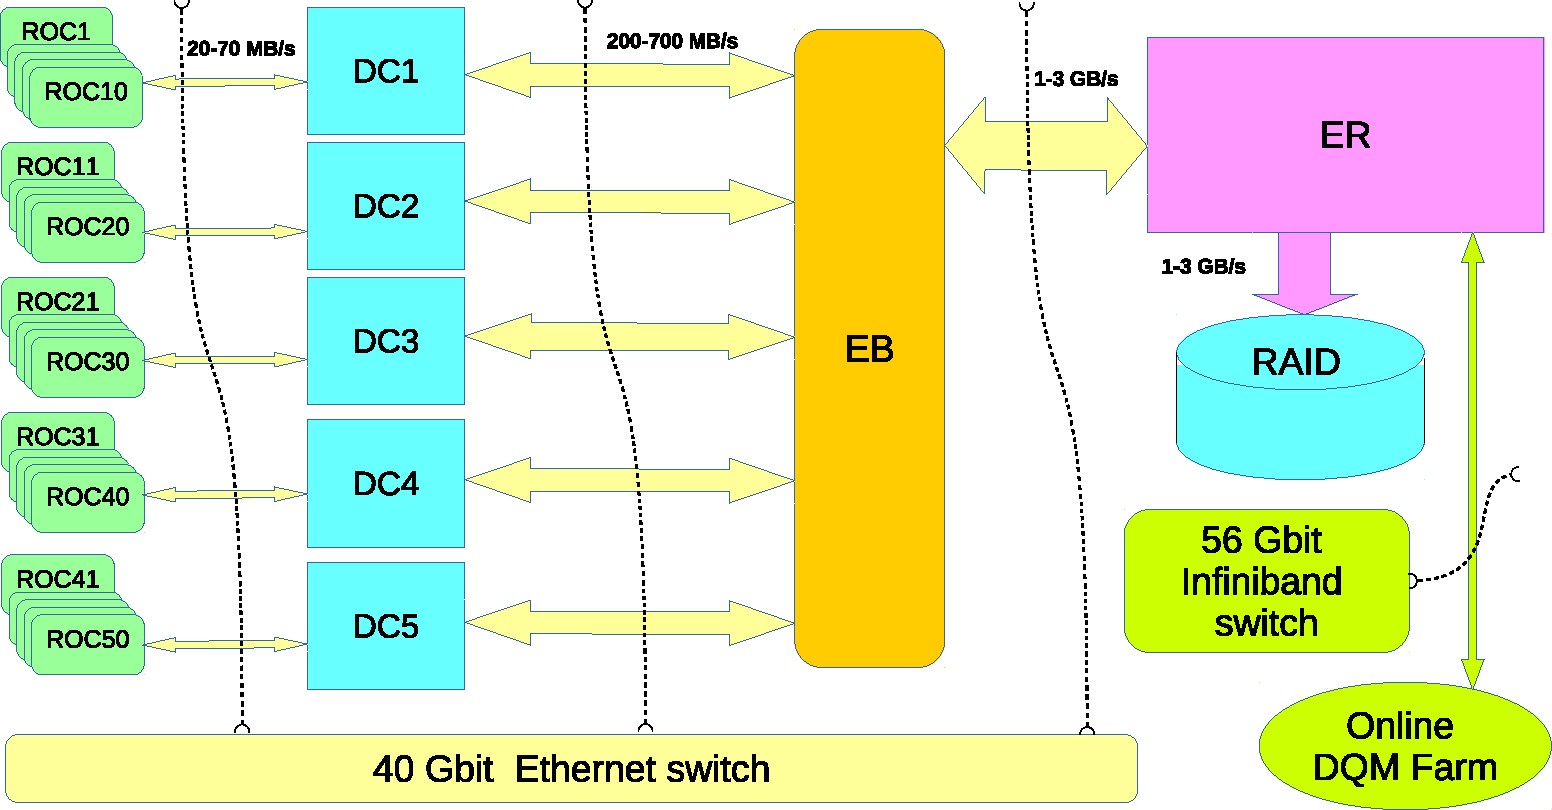
\includegraphics[width=0.75\textwidth]{figures/DAQ_coda.pdf}  
\caption{ \label{fig:CODA}
DAQ layout}

\end{center}
\end{figure}
